\documentclass[a4paper,10pt]{article}
\usepackage{float}
\usepackage{graphicx}
\usepackage[utf8]{inputenc}
\usepackage[spanish]{babel}
\usepackage{listings}
\usepackage{hyperref}
\usepackage{enumitem}
\usepackage{bookmark}
\usepackage{courier}
\usepackage[nocolor]{drawstack}
\usepackage{subfig}
\lstset{basicstyle=\footnotesize\ttfamily,breaklines=true}
\graphicspath{/imagenes,/Casos de prueba}

\title{		\textbf{Trabajo Práctico 1: \\
			Conjunto de instrucciones MIPS
			}}

\author{	Fabrizio Cozza, \textit{Padrón Nro. 97.402}                     \\
            \texttt{ fabrizio.cozza@gmail.com }                                              \\[2.5ex]
            Kevin Cajachuán, \textit{Padrón Nro. 98.725}                     \\
            \texttt{ kevincajachuan@hotmail.com }                                              \\[2.5ex]
            Luciano Giannotti, \textit{Padrón Nro. 97.215}                     \\
            \texttt{luciano\_giannotti@hotmail.com.ar}                                              \\[3.5ex]
	 \newline
            \normalsize{1er. Cuatrimestre de 2018}                                      \\
            \normalsize{66.20 Organización de Computadoras  $-$ Práctica Martes}  \\
            \normalsize{Facultad de Ingeniería, Universidad de Buenos Aires}            \\
       }
\date{}


\begin{document}
\maketitle
\thispagestyle{empty}   % quita el n�mero en la primer p�gina
\newpage

\section{Objetivos}

Este Trabajo Práctico tiene el fin de ayudarnos a familiarizarnos con el conjunto de instrucciones MIPS y el concepto de ABI, extendiendo un programa que resuelva el problema descripto en la siguiente sección.


\section{Programa}

El software de este trabajo está escrito en su mayoría en lenguaje C y permite dibujar \textbf{Julia Sets} o \textbf{Conjuntos de Julia} segun los parámetros que le pasamos por línea de comando.
Estos parámetros son la región del plano complejo: delimitada por un centro, un ancho y un alto; una semilla que afectará el calculo para cada pixel; la resolución y la salida ya sea por pantalla o por archivo. \\
La función en la cuál se encuentra la lógica de cómputo del fractal está escrita en MIPS con el fin de tener soporte nativo para NetBSD. \\
El formato a usar es  PGM o \textit{portable gray format}, que resulta útil para describir imágenes digitales en escala de grises.


\section{Implementación}

Una vez recibidos los parámetros, para dibujar el Julia Set el programa convierte cada píxel de la ventana a un punto en el plano complejo.
A ese punto se lo eleva al cuadrado y le suma la semilla mencionada en la sección anterior. Esto se repite hasta que el valor absoluto del resultado sea menor a 2, en cuyo caso se toma la cantidad de iteraciones y se imprime en el archivo PGM, representando el nivel de blanco de ese píxel.

\subsection{Funciones implementadas}
\subsubsection{mips32\_plot}
Esta función es la que se encarga de hacer los cálculos, para luego poder ir imprimiendo el valor de cada píxel en un archivo. \\
El único parámetro que recibe es un struct definido como \textit{param\_t} en el que se encuentran todos los datos necesarios para que la función realice su tarea, los cuales se obtienen de los parámetros pasados por el usuario por línea de comandos. \\
Esta función no devuelve nada ya que solo se dedica a hacer cálculos e imprimir. \\
El stack frame de esta función se muestra a continuación, en el cuál en cada dirección de memoria se indica qué variable está guardada.

\begin{center}
\begin{drawstack}
	\startframe
	\padding{1}{} \cellcom{60}
	\cell{ra} \cellcom{56}
	\cell{fp} \cellcom{52}
	\cell{gp} \cellcom{48}
	\finishframe{SRA}
	\startframe
	\cell{zi} \cellcom{44}
	\cell{zr} \cellcom{40}
	\cell{ci} \cellcom{36}
	\cell{cr} \cellcom{32}
	\finishframe{FRA}
	\startframe
	\cell{c} \cellcom{28}
	\cell{x} \cellcom{24}
	\cell{y} \cellcom{20}
	\cell{fd} \cellcom{16}
	\finishframe{LTA}
	\startframe
	\padding{1}{} \cellcom{12}
	\padding{1}{} \cellcom{8}
	\padding{1}{} \cellcom{4}
	\padding{1}{} \cellcom{0}
	\finishframe{ABA}
\end{drawstack}
\end{center}

\subsubsection{my\_fprintf}
Esta función imprime en un archivo llamando a la syscall \textit{write}, por lo que los parámetros que recibe son los mismo que recibe esta syscall: file descriptor del archivo, lo que se quiere escribir, y cuánto se quiere escribir. Finalmente devuelve la cantidad de bytes que se escribió la igual que la syscall. \\
El stack frame de esta función se muestra a continuación.

\begin{center}
\begin{drawstack}
	\startframe
	\padding{1}{} \cellcom{36}
	\cell{ra} \cellcom{32}
	\cell{fp} \cellcom{28}
	\cell{gp} \cellcom{24}
	\finishframe{SRA}
	\startframe
	\cell{total} \cellcom{20}
	\cell{n} \cellcom{16}
	\finishframe{LTA}
	\startframe
	\padding{1}{} \cellcom{12}
	\padding{1}{} \cellcom{8}
	\padding{1}{} \cellcom{4}
	\padding{1}{} \cellcom{0}
	\finishframe{ABA}
\end{drawstack}
\end{center}

\subsubsection{my\_strlen}
Esta función calcula la longitud de una cadena, recibiendo como parámetro la cadena y devolviendo la longitud. \\
El stack frame de la función se muestra a continuación. Al ser una función \textit{leaf}, no fue necesario tener un ABA ni salvar el registro \textit{ra}.
\begin{center}
\begin{drawstack}
	\startframe
	\cell{fp} \cellcom{4}
	\cell{gp} \cellcom{0}
	\finishframe{SRA}
\end{drawstack}
\end{center}

\subsubsection{int\_to\_str}
Esta función convierte un número a una cadena, llamando para realizar esto a dos funciones: \textit{dig\_to\_char} y \textit{put\_end}. Lo único que recibe la función es el número que se quiere convertir y no devuelve nada. \\
El stack frame se muestra a continuación.

\begin{center}
\begin{drawstack}
	\startframe
	\padding{1}{} \cellcom{36}
	\cell{ra} \cellcom{32}
	\cell{fp} \cellcom{28}
	\cell{gp} \cellcom{24}
	\finishframe{SRA}
	\startframe
	\cell{index} \cellcom{20}
	\cell{number} \cellcom{16}
	\finishframe{LTA}
	\startframe
	\padding{1}{} \cellcom{12}
	\padding{1}{} \cellcom{8}
	\padding{1}{} \cellcom{4}
	\padding{1}{} \cellcom{0}
	\finishframe{ABA}
\end{drawstack}
\end{center}

\subsubsection{dig\_to\_char}
Esta función recibe un número que se quiere convertir a cadena, un array para ir guardando los caracteres de cada dígito del número y el índice actual en el que hay que ir guardando cada caracter. Esta función se llama recursivamente para ir obteniendo los dígitos del número e ir guardandolos en el array. Como esto es lo único que realiza, la función no devuelve nada. \\
A continuación se muestra el stack frame de esta función.

\begin{center}
\begin{drawstack}
	\startframe
	\padding{1}{} \cellcom{36}
	\cell{ra} \cellcom{32}
	\cell{fp} \cellcom{28}
	\cell{gp} \cellcom{24}
	\finishframe{SRA}
	\startframe
	\padding{1}{} \cellcom{20}
	\cell{r} \cellcom{16}
	\finishframe{LTA}
	\startframe
	\padding{1}{} \cellcom{12}
	\padding{1}{} \cellcom{8}
	\padding{1}{} \cellcom{4}
	\padding{1}{} \cellcom{0}
	\finishframe{ABA}
\end{drawstack}
\end{center}

\subsubsection{put\_end}
Esta función lo único que hace es poner el caracter \textbackslash0 al final del array en que se guardaron los dígitos del número, para poder imprimirlo más adelante. Por esta razón esta función recibe como parámetros el array y el índice en el que se tiene que guardar el caracter \textbackslash0 y no devuelve ningún valor. \\
El stack frame se muestra a continuación. Por la misma razón que en la función \textit{my\_strlen}, no es necesario tener un ABA ni salvar \textit{ra}.

\begin{center}
\begin{drawstack}
	\startframe
	\cell{fp} \cellcom{4}
	\cell{gp} \cellcom{0}
	\finishframe{SRA}
\end{drawstack}
\end{center}

\section{Pruebas}
Como estamos probando imagenes, las pruebas las realizamos a ojo, comparandolas con las imagenes provistas como ejemplo en el enunciado y otras obtenidas con un generador online (\url{http://usefuljs.net/fractals/}). \\
Las imagenes de prueba se generaron corriendo el archivo \textbf{test.sh}. \\
Como resultado de los test, las imagenes generadas por el método genérico y el método MIPS32, son exactamente iguales, ya que al compararlas con el comando \textit{diff}, no hay diferencias entre ellas. \\
Los comandos mostrados en las siguientes subsecciones son para obtener las imágenes con el método MIPS32. Para obtener las imagenes con el método genérico únicamente hay que borrar el flag -m.

\subsubsection{Parámetros por defecto}
Esta prueba se realizó para verificar que la imagen obtenida sin pasar parámetros en la linea de comandos es la correcta. \\
El comando para obtener la imagen mostrada a continuación es:

\begin{lstlisting}[frame = single, language = bash, numbers=none]
$ ./tp1 -o gen1.pgm -m mips32
\end{lstlisting}

\begin{figure}[H]
 \centering
    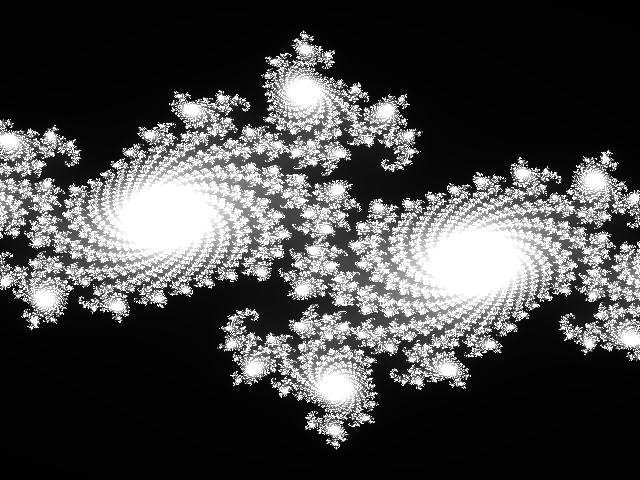
\includegraphics[width=0.5\textwidth]{../img_informe/uno.png}
\end{figure}

\subsubsection{Cambio de centro y zoom}
Esta prueba se realizó para verificar que la imagen obtenida cambiando los parámetros de altura, ancho y centro es la correcta. \\
El comando para obtener la imagen mostrada a continuación es:

\begin{lstlisting}[frame = single, language = bash, numbers=none]
$ ./tp1 -c 0.282-0.007i -w 0.005 -H 0.005 -o gen2.pgm -m mips32
\end{lstlisting}

\begin{figure}[H]
 \centering
    
\includegraphics[width=0.5\textwidth]{../img_informe/dos.png}
\end{figure}

\subsubsection{Cambio de ancho y altura}
Esta prueba se realizó para verificar que la imagen obtenida cambiando los parámetros de ancho y altura es la correcta. \\
Se prueba nuevamente los parámetros de ancho y altura para probar si son independientes del parámetro de centro. \\
El comando para obtener la imagen mostrada a continuación es:

\begin{lstlisting}[frame = single, language = bash, numbers=none]
$ ./tp1 -w 1 -H 1 -o gen3.pgm -m mips32
\end{lstlisting}

\begin{figure}[H]
 \centering
    
\includegraphics[width=0.5\textwidth]{../img_informe/tres.png}
\end{figure}

\subsubsection{Cambio de resolución}
Esta prueba se realizó para verificar que la imagen obtenida cambiando el parámetro de resolución es la correcta. \\
El comando para obtener la imagen mostrada a continuación es:

\begin{lstlisting}[frame = single, language = bash, numbers=none]
$ ./tp1 -r 8x6 -o gen4.pgm -m mips32
\end{lstlisting}

\begin{figure}[H]
 \centering
    
\includegraphics[width=0.5\textwidth]{../img_informe/cuatro.png}
\end{figure}

\subsubsection{Cambio de seed}
Esta prueba se realizó para verificar que la imagen obtenida cambiando el parámetro de seed es la correcta. \\
El comando para obtener la imagen mostrada a continuación es:

\begin{lstlisting}[frame = single, language = bash, numbers=none]
$ ./tp1 -0.157-1.041i -o gen5.pgm -m mips32
\end{lstlisting}

\begin{figure}[H]
 \centering
    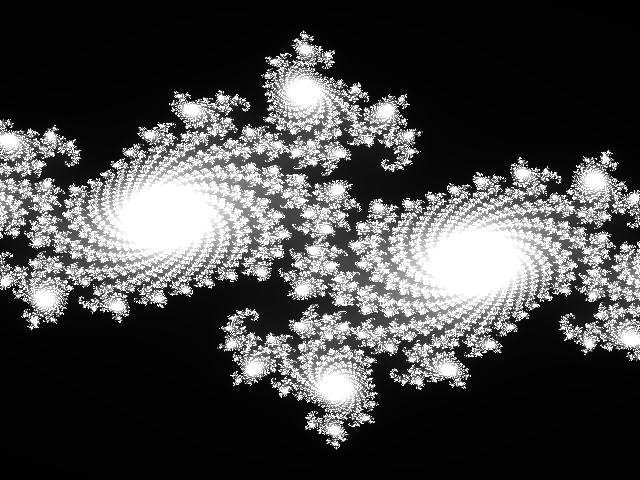
\includegraphics[width=0.5\textwidth]{../img_informe/uno.png}
\end{figure}

\subsubsection{Caso extremo}
Esta prueba se realizó para verificar que no ocurren problemas de dibujado en casos
extremos. Es difícil observarla en el informe por lo que decidimos no colocarla. Sin embargo los archivos se encuentran en el directorio Pruebas dentro del directorio del TP con los nombres \textit{gen6.pgm} y \textit{mips6.pgm}.\\
El comando para obtener las imagenes es:

\begin{lstlisting}[frame = single, language = bash, numbers=none]
$ -r 800x1 -o gen6.pgm -m mips32
\end{lstlisting}

\section{Compilación}

Como hay un archivo \textit{Makefile} que realiza la compilación, el único comando que hay que escribir en la terminal para compilarlo es:

\begin{lstlisting}[frame = single, language = bash, numbers=none]
$ make
\end{lstlisting}

\section{Código S}

En esta sección se muestra el código de la función mips32\_plot.

\lstinputlisting[basicstyle=\ttfamily\scriptsize,breaklines=true]{../mips32_plot.S}

\newpage

\section{Bibliografía}
\begin{enumerate}
\item GXemul. \\ http://gavare.se/gxemul/.
\item The NetBSD project. \\
	http://www.netbsd.org/.
\item Conjunto de Julia \\ 
	http://es.wikipedia.org/wiki/Conjunto\_de\_Julia (Wikipedia).
\item PGM format specification.\\
	http://netpbm.sourceforge.net/doc/pgm.html.
\item Generador de fractales. \\
	http://usefuljs.net/fractals/
\item GIMP. \\
	https://www.gimp.org/
\item System V Application Binary Interface. \\
	http://math-atlas.sourceforge.net/devel/assembly/mipsabi32.pdf
\end{enumerate}

\end{document}